\documentclass{article}
\usepackage[T1]{fontenc}
\usepackage{lmodern}
\usepackage{graphicx}
\usepackage{amsmath,amssymb}
\usepackage[a4paper,margin=2cm]{geometry}
\usepackage[absolute,overlay]{textpos}
\setlength{\TPHorizModule}{1mm}
\setlength{\TPVertModule}{1mm}
\usepackage[indonesian]{babel}
\usepackage{hyperref}
\setlength{\emergencystretch}{2em}
% unit: Halaman 45

\begin{document}

% === Halaman 45 (python/native) ===

• Kesalahan 1-bit pada blok plainteks hanya mempengaruhi blok cipherteks yang 

berkoresponden saja; begitu pula pada proses dekripsi, kesalahan 1-bit pada blok 

cipherteks hanya mempengaruhi blok plainteks yang bersangkutan saja.

• Karakteristik kesalahan semacam ini cocok untuk transmisi analog yang di-

digitisasi, seperti suara atau video, yang dalam hal ini kesalahan 1-bit dapat 

ditolerir, tetapi penjalaran kesalahan tidak dibolehkan.

45

% deskripsi: gambar native xref 189
\noindent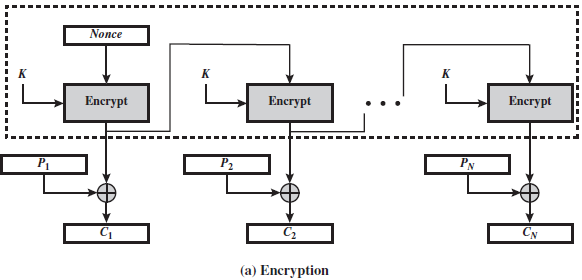
\includegraphics[width=0.85\textwidth]{../../images/python/page_045_img_01.png}

% deskripsi: gambar native xref 190
\noindent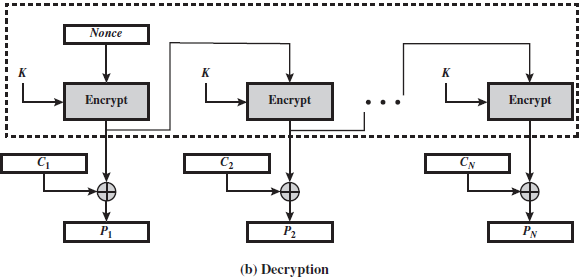
\includegraphics[width=0.85\textwidth]{../../images/python/page_045_img_02.png}

\end{document}
